\usepackage{cite}
% provides various features to facilitate writing math formulas and to improve the typographical quality of their output.
\usepackage{amsmath}
% \usepackage[cmex10]{amsmath}
\interdisplaylinepenalty=2500
\usepackage{amssymb,amsfonts}
\usepackage{algorithmic}
\usepackage{graphicx}
% \usepackage{graphicx}
\usepackage{textcomp}
\usepackage{xcolor}

% formatting from IEEE conference. Needs to be fitted with our natbib
\def\BibTeX{{\rm B\kern-.05em{\sc i\kern-.025em b}\kern-.08em
		T\kern-.1667em\lower.7ex\hbox{E}\kern-.125emX}}

%%%%%%%%%%%%%%%%%%%%%%%%
%Article stuff
%%%%%%%%%%%%%%%%%%%%%%%%
% This package serves to balance the column lengths on the last page of the document.
% please, insert \balance command in the left column of the last page
\usepackage{balance}
\usepackage{supertabular}
\usepackage{paralist}
\usepackage{booktabs}

%% to enable \thank command
\IEEEoverridecommandlockouts 
% to typeset algorithms
\usepackage{algorithm}
%\usepackage{algpseudocode}
% to typeset code fragments
\usepackage{listings}
% to make an accent \k be available
\usepackage[T1]{fontenc}
% por urls typesetting and breaking
\usepackage{url}
% for vertical merging table cells
\usepackage{multirow}
\usepackage{siunitx}


%%%%%%%%%%%%%%%%%%%%%%%%
%Mixed packages
%%%%%%%%%%%%%%%%%%%%%%%%
\usepackage[hidelinks]{hyperref}
\usepackage{graphicx}
\usepackage[textsize=scriptsize]{todonotes}
\usepackage{glossaries}
\usepackage[numbers]{natbib}
\usepackage{subcaption}
\bibliographystyle{plainnat}

\let\labelindent\relax %Needed before enumitem to avoid error with IEEE template
\usepackage{enumitem}
% Encoding %
\usepackage[utf8]{inputenc}
\usepackage{enumitem}
\usepackage{framed}


%%%%%%%%%%%%%%%%%%%%%%%%
%Figures
%%%%%%%%%%%%%%%%%%%%%%%%

\usepackage{tikz}
\usepackage{pgfplots}

% Tables %
\usepackage{tabularx}
\usepackage{xltabular}
\newcolumntype{Y}{>{\centering\arraybackslash}X}
\usepackage{booktabs} % for professional tables
\usepackage{tikz}
\usetikzlibrary{positioning}
\usepackage{longtable}
\usepackage{makecell}
\usetikzlibrary{shapes.geometric, arrows}
\usetikzlibrary{matrix,positioning,arrows.meta,arrows}

\tikzset{my arrow/.style={-latex},
	set@com@col/.style={},set@com@col@aryarg/.style={column #1/.style={set@com@col}},
	set@com@row/.style={},set@com@row@aryarg/.style={row #1/.style={set@com@row}},
	set common column/.style 2 args={set@com@col/.style={#2}, set@com@col@aryarg/.list={#1}},
	set common row/.style 2 args={set@com@row/.style={#2}, set@com@row@aryarg/.list={#1}},
}

%%%%%%%%%%%%%%%%%%%%%%%%
%Defines
%%%%%%%%%%%%%%%%%%%%%%%%

\newtheorem{definition}{\textbf{Definition}}

% Autoref
\def\sectionautorefname{Section}
\def\subsectionautorefname{Section}
\def\subsubsectionautorefname{Section}
\def\figureautorefname{Fig.}
\def\definitionautorefname{Definition}

% Plates
\usepackage{amstext}
\usepackage{tikz}
\usetikzlibrary{arrows,decorations.pathmorphing,fit,positioning}

\newcommand{\dir}{\text{Dirichlet}}
\newcommand{\mult}{\text{Multinomial}}


% Glossaries
\newacronym{lda}{LDA}{latent Dirichlet allocation}
\newacronym{NLP}{NLP}{Natural Language Processing}
\newacronym{tf-idf}{tf-idf}{Term Frequency-Inverse Document Frequency}
\newacronym{lm}{LM}{Language Model}
\newacronym{vi}{VI}{Variational Inference}
\newacronym{pr}{PR}{PageRank}
\newacronym{ppr}{PPR}{Personalized PageRank}
\newacronym{bm25}{BM25}{Okapi Best Matching 25}
\newacronym{ir}{IR}{Information Retrieval}
\newacronym{map}{MAP}{Mean Average Precision}
\newacronym{dag}{DAG}{Directed Acyclic Graph}

%Glossary changes
%%%%%%%%%%%%%%%%%%%%%%%%
% Switch off hyperlinks for all uses of \gls etc.
% Hyperlinks will be inserted manually in the custom display style
\setkeys{glslink}{hyper=false}

\renewcommand*{\CustomAcronymFields}{%
	name={\the\glsshorttok},%
	description={\the\glslongtok},%
}

\renewcommand*{\SetCustomDisplayStyle}[1]{%
	\defglsentryfmt[#1]{%
		\ifdefempty\glscustomtext
		{%
			\ifglsused\glslabel
			{% subsequent use
				% Assuming all acronyms are written in upper case, so
				% not bother to check for case changes.
				\glsifplural
				{% subsequent use, plural
					\glshyperlink[\glsentryshortpl{\glslabel}]{\glslabel}%
				}%
				{% subsequent use, singular
					\glshyperlink[\glsentryshort{\glslabel}]{\glslabel}%
				}%
			}%
			{% first use
				\glsifplural
				{% first use, plural
					\glscapscase
					{% no case change
						\glstarget{\glslabel}{\glsentrylongpl{\glslabel}\glsinsert}%
						\space(\glsentryshortpl{\glslabel})%
					}%
					{% first letter upper case
						\glstarget{\glslabel}{\Glsentrylongpl{\glslabel}\glsinsert}%
						\space(\glsentryshortpl{\glslabel})%
					}%
					{% all caps
						\glstarget{\glslabel}{\MakeTextUppercase{%
								\glsentrylongpl{\glslabel}\glsinsert}}%
						\MakeTextUppercase{\space(\glsentryshortpl{\glslabel})}%
					}%
				}%
				{% first use, singular
					\glscapscase
					{% no case change
						\glstarget{\glslabel}{\glsentrylong{\glslabel}\glsinsert}%
						\space(\glsentryshort{\glslabel})%
					}%
					{% first letter upper case
						\glstarget{\glslabel}{\Glsentrylong{\glslabel}\glsinsert}%
						\space(\glsentryshort{\glslabel})%
					}%
					{% all caps
						\glstarget{\glslabel}{\MakeTextUppercase{%
								\glsentrylong{\glslabel}\glsinsert}}%
						\MakeTextUppercase{\space(\glsentryshort{\glslabel})}%
					}%
				}%
			}%
		}%
		{% \glsdisp used
			\ifglsused\glslabel
			{% subsequent use
				\glshyperlink[\glscustomtext]{\glslabel}%
			}%
			{% first use
				\glstarget{\glslabel}{\glscustomtext}%
			}%
		}%
	}%
}

\SetCustomStyle


\title% optional, use only with long paper titles
{Integrating News Article Metadata into Topic Models}
% \subtitle{}  % could also be a conference name

\date{\today}

\author % optional, use only with lots of authors
{Rasmus Engesgaard Christensen, Peter Langballe Erichsen, and \\ Dennis Højbjerg Rose
}
% - Give the names in the same order as they appear in the paper.
% - Use the \inst{?} command only if the authors have different
%   affiliation. See the beamer manual for an example

\institute[
%  {\includegraphics[scale=0.2]{aau_segl}}\\ %insert a company, department or university logo
  Dept.\ of Computer Science\\
  Aalborg University\\
  Denmark
] % optional - is placed in the bottom of the sidebar on every slide
{% is placed on the title page
  Department of Computer Science\\
  Aalborg University\\
  Denmark

  %there must be an empty line above this line - otherwise some unwanted space is added between the university and the country (I do not know why;( )
}


% specify a logo on the titlepage (you can specify additional logos an include them in 
% institute command below
\pgfdeclareimage[height=1.5cm]{titlepagelogo}{AAUgraphics/aau_logo_new} % placed on the title page
%\pgfdeclareimage[height=1.5cm]{titlepagelogo2}{graphics/aau_logo_new} % placed on the title page
\titlegraphic{% is placed on the bottom of the title page
  \pgfuseimage{titlepagelogo}
%  \hspace{1cm}\pgfuseimage{titlepagelogo2}
}

\begin{document}
% the titlepage
{\aauwavesbg%
\begin{frame}[plain,noframenumbering] % the plain option removes the sidebar and header from the title page
  \titlepage
\end{frame}}
%%%%%%%%%%%%%%%%

% TOC
\begin{frame}[noframenumbering]{Agenda}{}
\setcounter{tocdepth}{1}
\tableofcontents
\end{frame}
%%%%%%%%%%%%%%%%
\subsection{Language Model}
\begin{frame}{\insertsubsection}{Information retrieval goal}
    \begin{itemize}
        \item We want to find relevant documents based on words in a query
        \begin{equation*}\label{eq:query_prob}
	        P(q|d) = \prod_{w \in q} P(w|d)
        \end{equation*}
    \end{itemize}
\end{frame}

\begin{frame}{\insertsubsection}{Explanation}
    \only<1>{
    \begin{equation*}\label{eq:word_prob}
    	P(w|d) = \frac{N_d}{N_d + \lambda} \cdot \frac{tf(w,d)}{N_d} + (1 - \frac{N_d}{N_d + \lambda}) \cdot \frac{tf(w,D)}{N_D}
    \end{equation*}
    \begin{itemize}
        \item $d$ = document
        \item $N_d$ = Number of words in $d$
        \item $\lambda$ is the average document length 
        \item $D$ = Corpus
    \end{itemize}
    }
    \only<2>{
    \begin{equation*}\label{eq:word_prob}
    	P(w|d) = \underbrace{\frac{N_d}{N_d + \lambda}}_{\text{weight term}} \cdot \frac{tf(w,d)}{N_d} + \underbrace{(1 - \frac{N_d}{N_d + \lambda})}_{\text{inverse weight term}} \cdot \frac{tf(w,D)}{N_D}
    \end{equation*}
    \begin{itemize}
        \item $d$ = document
        \item $N_d$ = Number of words in $d$
        \item $\lambda$ is the average document length 
        \item $D$ = Corpus
    \end{itemize}
    }
    \only<3>{
    \begin{equation*}\label{eq:word_prob}
    	P(w|d) = \underbrace{\frac{N_d}{N_d + \lambda}}_{\text{weight term}} \cdot \underbrace{\frac{tf(w,d)}{N_d}}_{\text{\% of w in d}} + \underbrace{(1 - \frac{N_d}{N_d + \lambda})}_{\text{inverse weight term}} \cdot \underbrace{\frac{tf(w,D)}{N_D}}_{\text{\% w in D}}
    \end{equation*}
    \begin{itemize}
        \item $d$ = document
        \item $N_d$ = Number of words in $d$
        \item $\lambda$ is the average document length 
        \item $D$ = Corpus
    \end{itemize}
    }
    \only<4>{
    \begin{equation*}\label{eq:word_prob}
    	P(w|d) = \underbrace{\frac{N_d}{N_d + \lambda}}_{\text{weight term}} \cdot \underbrace{\frac{tf(w,d)}{N_d}}_{\text{\% of w in d}} + \underbrace{(1 - \frac{N_d}{N_d + \lambda})}_{\text{inverse weight term}} \cdot \underbrace{\frac{tf(w,D)}{N_D}}_{\text{\% w in D}}
    \end{equation*}
    \begin{itemize}
        \item $d$ = document
        \item $N_d$ = Number of words in $d$
        \item $\lambda$ is the average document length 
        \item $D$ = Corpus
    \end{itemize}
    }
    \only<5>{
        \begin{itemize}
            \item Favors high percentage of a word in a document or corpus
        \end{itemize}
    }
\end{frame}

\subsection{TF-IDF}
\begin{frame}{\insertsubsection}{Explanation}
    \only<1>{
    \begin{equation*}\label{eq:tfidf}
    	\text{tf-idf}(t, d, D) = \text{tf}(t, d) \cdot \text{idf}(t, D)
    \end{equation*}
    \begin{itemize}
        \item $t$ = Term
        \item $d$ = Document
        \item $D$ = Corpus
    \end{itemize}
    }
    \only<2>{
    \begin{equation*}\label{eq:tfidf}
    	\text{tf-idf}(t, d, D) = \text{tf}(t, d) \cdot log \frac{|\{d \in D\}|}{|\{d \in D : t \in d\}|}
    \end{equation*}
    }
\end{frame}

\begin{frame}{\insertsubsection}{Summary}
    \begin{itemize}
        \item Favors high usage of unique word(s) in a document or corpus
    \end{itemize}
\end{frame}


\subsection{BM25}
\begin{frame}{\insertsubsection}{Explanation}
    \only<1>{
    \begin{equation*}\label{eq:bm25}
    	\text{bm25}(d, q) = \sum_{i=1}^{n}\text{idf}(q_i) \cdot \frac{\text{tf}(q_i, d) \cdot (k_1 + 1)}{\text{tf}(q_i, d) + k_1 \cdot (1 - b + b \cdot \frac{|d|}{avgdl})}
    \end{equation*}
    \begin{itemize}
        \item $b$ adjust the sensitivity of varying document lengths
        \item $k_1$ adjust how quickly a term is saturated 
    \end{itemize}
    }
    
    \only<2>{
    \begin{equation*}\label{eq:bm25}
    	\text{bm25}(d, q) = \sum_{i=1}^{n}\text{idf}(q_i) \cdot \frac{\text{tf}(q_i, d) \cdot (1.5 + 1)}{\text{tf}(q_i, d) + 1.5 \cdot (1 - 0.75 + 0.75 \cdot \frac{|d|}{avgdl})}
    \end{equation*}
    }
\end{frame}

\begin{frame}{\insertsubsection}{Summary}
    \begin{itemize}
        \item Similar to tf-idf but with some other focus points
        \begin{itemize}
            \item Document length 
            \item Word saturation 
        \end{itemize}
    \end{itemize}
\end{frame}



\subsection{Combination of methods}
\begin{frame}{\insertsubsection}{How to combine?}
    \begin{figure}
    \centering
    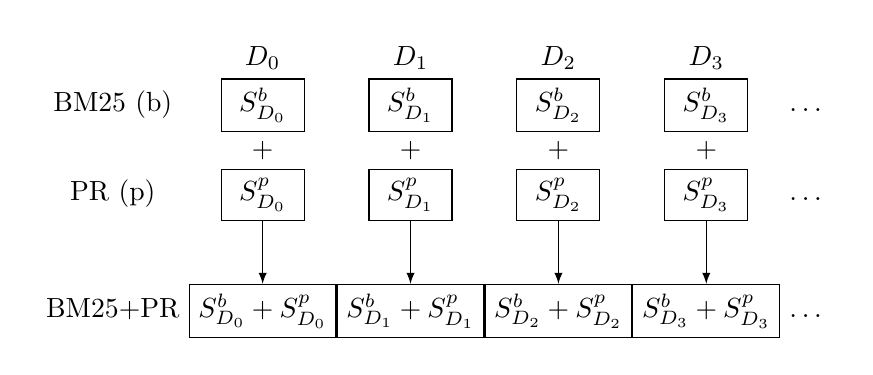
\begin{tikzpicture}
        \matrix [matrix of nodes,row sep=0mm, set common column={2,3,4,5,7}{nodes={rectangle,draw,minimum width=3em}}, set common row={1,3} {nodes={draw=none}}, ] (O)
        {
            & $D_0$ & $D_1$ & $D_2$ & $D_3$ &  \\
            BM25 (b) & $S^{b}_{D_0}$ & $S^{b}_{D_1}$ & $S^{b}_{D_2}$ & $S^{b}_{D_3}$ & \dots \\
            & + & + & + & + & \\
            PR (p) & $S^{p}_{D_0}$ & $S^{p}_{D_1}$ & $S^{p}_{D_2}$ & $S^{p}_{D_3}$ & \dots \\[8mm]
            BM25+PR & $S^{b}_{D_0} + S^{p}_{D_0} $ & $S^{b}_{D_1} + S^{p}_{D_1} $ & $S^{b}_{D_2} + S^{p}_{D_2} $ & $S^{b}_{D_3} + S^{p}_{D_3} $ &  \dots \\
        };
        \foreach\x in{2,3,4,5}{\draw[my arrow] (O-4-\x) to (O-5-\x);}
    \end{tikzpicture}
\end{figure}
    \vspace{0.5cm}
    \only<2>{
        \begin{itemize}
            \item $ t \cdot A + (1-t) \cdot B $
        \end{itemize}
    }
\end{frame}

\section{Query Generation}
\begin{frame}{\insertsection}{Types of queries}
    \begin{itemize}
        \item Document query
        \begin{itemize}
            \item Specificity - Finding a specific document
        \end{itemize}
        \item Topic query
        \begin{itemize}
            \item Generality - Finding topic relevant documents
        \end{itemize}
    \end{itemize}
\end{frame}

\subsection{Document Query}
\begin{frame}{\insertsubsection}{Generation}
    \tikzstyle{document} = [circle, rounded corners ,text centered, draw=black]
\tikzstyle{corpus} = [draw,thick,minimum width=1cm,minimum height=4cm]
\tikzstyle{tf-idf} = [draw,thick,minimum width=1cm,minimum height=1cm]

\begin{tikzpicture}
    \node [fill=gray, label={Corpus}] (corpus) at (0,0) [corpus] {};
    \onslide<2->{
        \node [document, label={d}] (doc) at (2, 0) {};
        \draw [line width=0.25mm, ->] (0,0) -> (1.85,0) node [right] {};
    };
    \onslide<3->{
        \node [fill=gray, label={tf-idf}] (tf-idf) at (4,0) [tf-idf] {};
        \draw [line width=0.25mm, ->] (doc) -> (tf-idf)  {};
    };
    \onslide<4->{
        \node [document, label={Query}] (Query) at  (7, 0) {};
        \draw [line width=0.25mm, ->] (tf-idf) -- node[below] {$1$-$4$ words} ++(2.6,0) -- (Query);
    };
    \onslide<5->{
        \path (doc) edge[bend right=75, dashed, <-] node [left] {} (Query);
    }
\end{tikzpicture}
\end{frame}

\subsection{Topic Query}
\begin{frame}{\insertsubsection}{Generation}
    \tikzstyle{document} = [circle, rounded corners ,text centered, draw=black]
\tikzstyle{topic} = [draw,thick,minimum width=1cm,minimum height=4cm]
\tikzstyle{tf-idf} = [draw,thick,minimum width=1cm,minimum height=1cm]

\begin{tikzpicture}
    \node [fill=gray, label={Topics}] (topic) at (0,0) [topic] {};
    \onslide<2->{
        \node [document, label={t}] (top) at (2, 0) {};
        \draw [line width=0.25mm, ->] (0,0) -> (top) node [right] {};
    };
    \onslide<3->{
        \node [fill=gray, label={topic-document dist.}] (dist) at (4,0) [tf-idf] {};
        \draw [line width=0.25mm, ->] (top) -> (dist)  {};
    };
    \onslide<4->{
        \node [document, label={Documents}] (documents) at  (7, 0) {};
        \draw [line width=0.25mm, ->] (dist) -- node[below] {1-4 doc} ++(2.5,0) -- (documents);
    };
    \onslide<5->{
        \node [document, label=below:Query] (query) at  (7, -2) {};
        \draw [line width=0.25mm, ->] (documents) -- node[right] {1 word} ++(0,-1.75) -- (query);
    };
\end{tikzpicture}
    \only<6>{
        \begin{itemize}
            \item Sample the topic-word distribution instead
        \end{itemize}
    }
\end{frame}
\subsection{\acrlong{pam}}

\begin{frame}{\insertsubsection}{\gls{dag} structure}
    \begin{itemize}
    	\item<1-> Hierarchical topic model, capturing correlation between topics
    	\item<2-> Topic distributions can include other topics as well as words
    \end{itemize}
	
	\only<3->{
	\begin{figure}
		\centering
		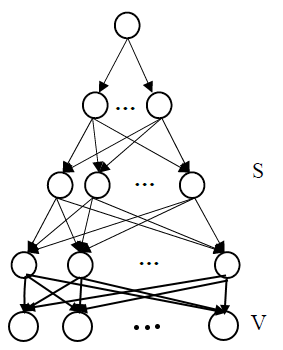
\includegraphics[width=0.35 \textwidth]{../figures/pachinko_dag}
	\end{figure}}
\end{frame}

\begin{frame}{\insertsubsection}{Plate Notation}
	%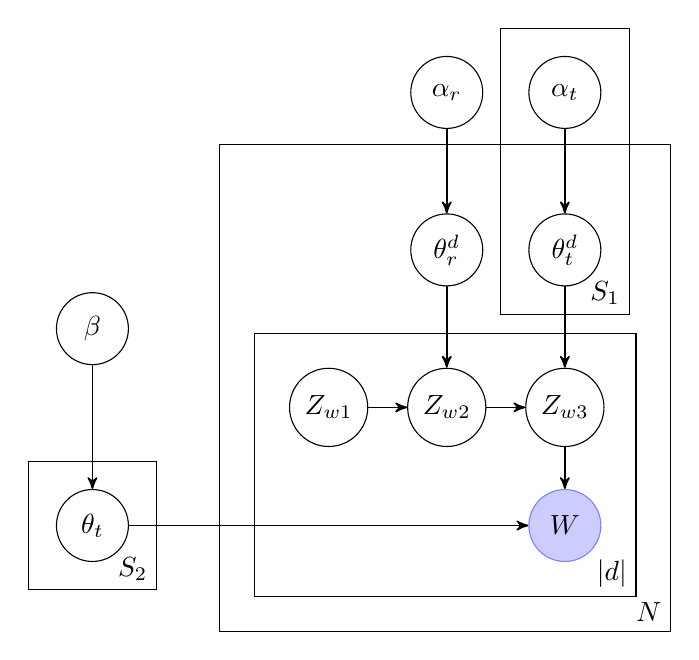
\begin{tikzpicture}
	[
	observed/.style={minimum size=26pt,circle,draw=blue!50,fill=blue!20},
	unobserved/.style={minimum size=26pt,circle,draw},
	post/.style={->,>=stealth',semithick},
	]
	
	\node (w-j) [observed] at (0,0) {$W$};
	\node (z-3) [unobserved, above of= w-j, node distance=1.5cm] {$Z_{w3}$};
	\node (z-2) [unobserved, left of= z-3, node distance=1.5cm] {$Z_{w2}$};
	\node (z-1) [unobserved, left of= z-2, node distance=1.5cm] {$Z_{w1}$};
	
	\node (theta_r) [unobserved, above of= z-2, node distance=2cm] {$\theta_r^d$};
	\node (alpha_r) [unobserved, above of= theta_r , node distance=2cm] {$\alpha_r$};
	
	\node (theta_k) [unobserved, above of= z-3, node distance=2cm] {$\theta_{t}^d$};
	\node (alpha_k) [unobserved, above of= theta_k , node distance=2cm] {$\alpha_{t}$};
	
	\node (theta_s2) [unobserved, left of=w-j , node distance=6cm] {$\theta_{t}$};
	\node (beta) [unobserved, above of=theta_s2 , node distance=2.5cm] {$\beta$};
	
	\path
	(z-3) edge [post] (w-j)
	(z-2) edge [post] (z-3)
	(z-1) edge [post] (z-2)
	
	(theta_r) edge [post] (z-2)
	(alpha_r) edge [post] (theta_r)
	
	(theta_k) edge [post] (z-3)
	(alpha_k) edge [post] (theta_k)
	
	(theta_s2) edge [post] (w-j)
	(beta) edge [post] (theta_s2)
	;
	
	\node [draw,fit=(w-j) (theta_r) (z-1), inner sep=25pt] (plate-context) {};
	\node [above left] at (plate-context.south east) {$N$};
	
	\node [draw,fit=(w-j) (z-1), inner sep=12.5pt] (plate-token) {};
	\node [above left] at (plate-token.south east) {$|d|$};
	
	\node [draw,fit=(theta_s2), inner sep=10pt] (plate-token) {};
	\node [above left] at (plate-token.south east) {$S_2$};
	
	\node [draw,fit=(theta_k) (alpha_k), inner sep=10pt] (plate-token) {};
	\node [above left] at (plate-token.south east) {$S_1$};
\end{tikzpicture}

	\begin{figure}
			\centering
			\resizebox{0.45\columnwidth}{!}{%
			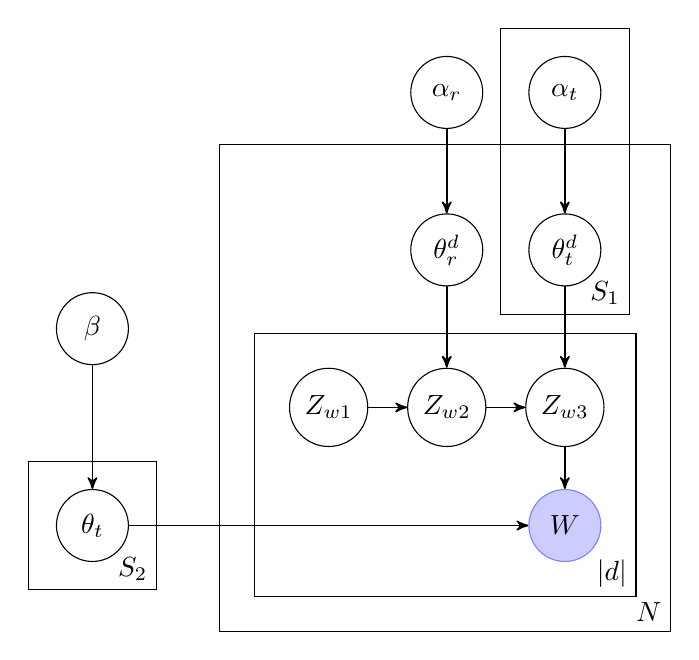
\begin{tikzpicture}
	[
	observed/.style={minimum size=26pt,circle,draw=blue!50,fill=blue!20},
	unobserved/.style={minimum size=26pt,circle,draw},
	post/.style={->,>=stealth',semithick},
	]
	
	\node (w-j) [observed] at (0,0) {$W$};
	\node (z-3) [unobserved, above of= w-j, node distance=1.5cm] {$Z_{w3}$};
	\node (z-2) [unobserved, left of= z-3, node distance=1.5cm] {$Z_{w2}$};
	\node (z-1) [unobserved, left of= z-2, node distance=1.5cm] {$Z_{w1}$};
	
	\node (theta_r) [unobserved, above of= z-2, node distance=2cm] {$\theta_r^d$};
	\node (alpha_r) [unobserved, above of= theta_r , node distance=2cm] {$\alpha_r$};
	
	\node (theta_k) [unobserved, above of= z-3, node distance=2cm] {$\theta_{t}^d$};
	\node (alpha_k) [unobserved, above of= theta_k , node distance=2cm] {$\alpha_{t}$};
	
	\node (theta_s2) [unobserved, left of=w-j , node distance=6cm] {$\theta_{t}$};
	\node (beta) [unobserved, above of=theta_s2 , node distance=2.5cm] {$\beta$};
	
	\path
	(z-3) edge [post] (w-j)
	(z-2) edge [post] (z-3)
	(z-1) edge [post] (z-2)
	
	(theta_r) edge [post] (z-2)
	(alpha_r) edge [post] (theta_r)
	
	(theta_k) edge [post] (z-3)
	(alpha_k) edge [post] (theta_k)
	
	(theta_s2) edge [post] (w-j)
	(beta) edge [post] (theta_s2)
	;
	
	\node [draw,fit=(w-j) (theta_r) (z-1), inner sep=25pt] (plate-context) {};
	\node [above left] at (plate-context.south east) {$N$};
	
	\node [draw,fit=(w-j) (z-1), inner sep=12.5pt] (plate-token) {};
	\node [above left] at (plate-token.south east) {$|d|$};
	
	\node [draw,fit=(theta_s2), inner sep=10pt] (plate-token) {};
	\node [above left] at (plate-token.south east) {$S_2$};
	
	\node [draw,fit=(theta_k) (alpha_k), inner sep=10pt] (plate-token) {};
	\node [above left] at (plate-token.south east) {$S_1$};
\end{tikzpicture}

			}
	\end{figure}
	\begin{itemize}
		\item Topic are sampled based on previous topics
	\end{itemize}
\end{frame}

\subsection{Taxonomy-Topic Model}

\begin{frame}{\insertsubsection}{Problems}
	Features needed to support taxonomy metadata:
	\begin{itemize}
		\item<1-> Hierarchical Structure
		\item<2-> Metadata Incorporation
		\item<3-> Partially Observed
		\item<4-> Multiple Taxonomies
	\end{itemize}
\end{frame}

\begin{frame}{\insertsubsection}{Metadata Incorporation}
	\begin{itemize}
		\item<1-> 1:1 mapping between topics and taxonomy entries
		\only<2>{\newline\begin{figure}
	\centering
	\resizebox{0.8\columnwidth}{!}{%
	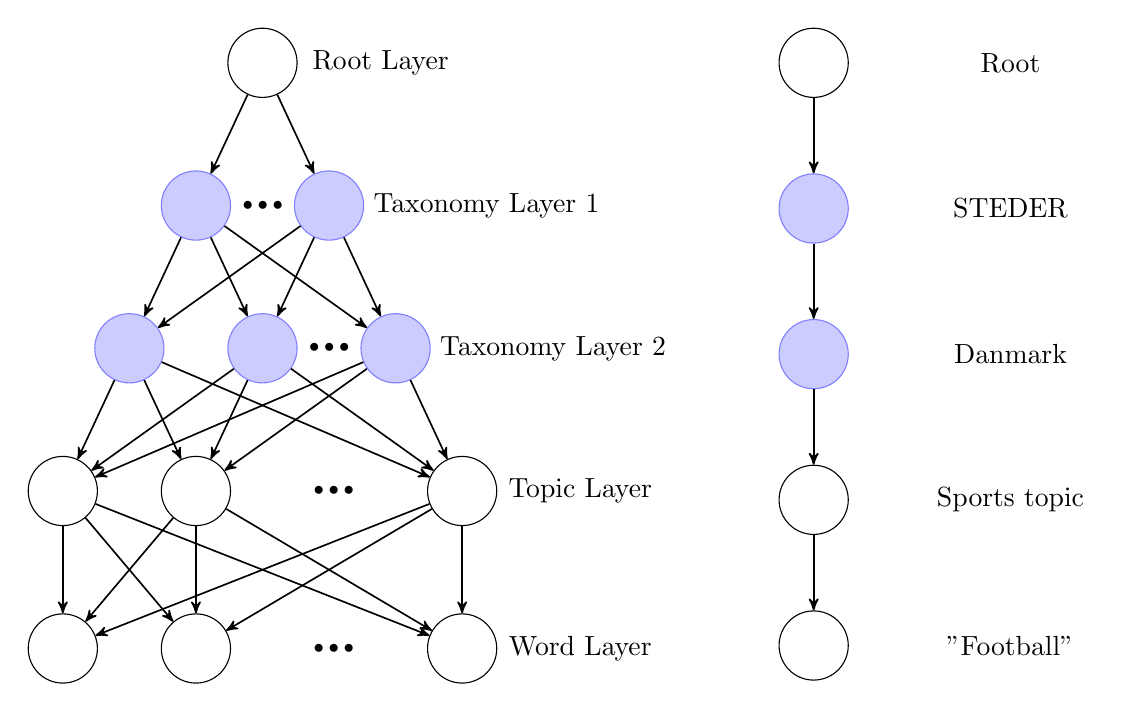
\begin{tikzpicture}
		[
		observed/.style={minimum size=25pt,circle,draw=blue!50,fill=blue!20},
		unobserved/.style={minimum size=25pt,circle,draw},
		post/.style={->,>=stealth',semithick},
		]
		% Layer 0
		\node (top) [unobserved] at (0,0) {};
		\node (topname) [right of = top, node distance=1.5cm] {Root Layer};
		
		% Layer 1
		\node (l11) [observed] at ([shift=({245:2 cm})]top) {};
		\node (l12) [observed] at ([shift=({295:2 cm})]top) {};
		\node (l1_dots) [right of = l11, node distance=0.85cm] {\scalebox{0.75}{$\bullet\bullet\bullet$}};
		\node (1name) [right of = l12, node distance=2cm] {Taxonomy Layer 1};
		
		% Layer 2
		\node (l21) [observed] at ([shift=({245:2 cm})]l11) {};
		\node (l22) [observed] at ([shift=({295:2 cm})]l11) {};
		\node (l23) [observed] at ([shift=({295:2 cm})]l12) {};
		\node (l2_dots) [right of = l22, node distance=0.85cm] {\scalebox{0.75}{$\bullet\bullet\bullet$}};
		\node (2name) [right of = l23, node distance=2cm] {Taxonomy Layer 2};
		
		% Layer 3
		\node (l31) [unobserved] at ([shift=({245:2 cm})]l21) {};
		\node (l32) [unobserved] at ([shift=({295:2 cm})]l21) {};
		\node (l33) [unobserved] at ([shift=({295:2 cm})]l23) {};
		\node (l2_dots) [right of = l32, node distance=1.75cm] {\scalebox{0.75}{$\bullet\bullet\bullet$}};
		\node (3name) [right of = l33, node distance=1.5cm] {Topic Layer};
		
		% Layer 4
		\node (l41) [unobserved] at ([shift=({270:2 cm})]l31) {};
		\node (l42) [unobserved] at ([shift=({270:2 cm})]l32) {};
		\node (l43) [unobserved] at ([shift=({270:2 cm})]l33) {};
		\node (l2_dots) [right of = l42, node distance=1.75cm] {\scalebox{0.75}{$\bullet\bullet\bullet$}};
		\node (4name) [right of = l43, node distance=1.5cm] {Word Layer};
		
		\path
		% Layer 0
		(top) edge [post] (l11)
		(top) edge [post] (l12)
		
		% Layer 1
		(l11) edge [post] (l21)
		(l11) edge [post] (l22)
		(l11) edge [post] (l23)
		(l12) edge [post] (l21)
		(l12) edge [post] (l22)
		(l12) edge [post] (l23)
		
		% Layer 2
		(l21) edge [post] (l31)
		(l21) edge [post] (l32)
		(l21) edge [post] (l33)
		(l22) edge [post] (l31)
		(l22) edge [post] (l32)
		(l22) edge [post] (l33)
		(l23) edge [post] (l31)
		(l23) edge [post] (l32)
		(l23) edge [post] (l33)
		
		% Layer 3
		(l31) edge [post] (l41)
		(l31) edge [post] (l42)
		(l31) edge [post] (l43)
		(l32) edge [post] (l41)
		(l32) edge [post] (l42)
		(l32) edge [post] (l43)
		(l33) edge [post] (l41)
		(l33) edge [post] (l42)
		(l33) edge [post] (l43)
		;
		
		
		\node (root) [unobserved, node distance=1.85cm] at (7,0) {};
		\node (rootname) [right of = root, node distance=2.5cm] {Root};
		
		\node (first) [observed, below of=root, node distance=1.85cm] {};
		\node (firstname) [right of = first, node distance=2.5cm] {STEDER};
		
		\node (second) [observed, below of=first, node distance=1.85cm] {};
		\node (secondname) [right of = second, node distance=2.5cm] {Danmark};
		
		\node (third) [unobserved, below of=second, node distance=1.85cm] {};
		\node (thirdname) [right of = third, node distance=2.5cm] {Sports topic};
		
		\node (fourth) [unobserved, below of=third, node distance=1.85cm] {};
		\node (fourthname) [right of = fourth, node distance=2.5cm] {"Football"};
		
		
		\path
		% Layer 0
		(root) edge [post] (first)
		(first) edge [post] (second)
		(second) edge [post] (third)
		(third) edge [post] (fourth)
		;
		
\end{tikzpicture}}
\end{figure}
}
	\end{itemize}
\end{frame}

\begin{frame}{\insertsubsection}{Metadata Incorporation}
	\begin{itemize}
		\item<1-> Restrict sampling from documents with known taxonomy
		\item<2-> Unobserved taxonomy sequences work like normal
		\item<3-> For documents with multiple sequences, we randomly choose one sequence for each word
	\end{itemize}
\end{frame}

\begin{frame}{\insertsubsection}{Plate Notation}
	\begin{columns}
		\begin{column}{0.45\textwidth}
			\begin{figure}
				\resizebox{\textwidth}{!}{%
					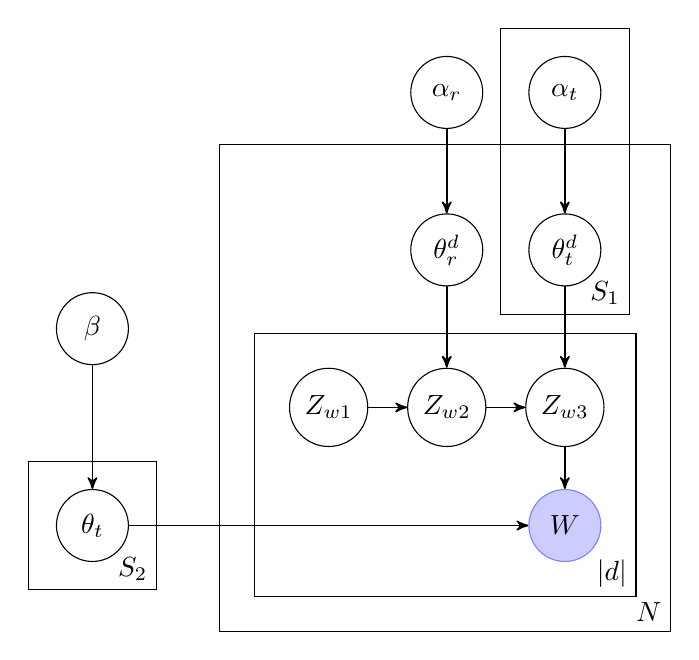
\begin{tikzpicture}
	[
	observed/.style={minimum size=26pt,circle,draw=blue!50,fill=blue!20},
	unobserved/.style={minimum size=26pt,circle,draw},
	post/.style={->,>=stealth',semithick},
	]
	
	\node (w-j) [observed] at (0,0) {$W$};
	\node (z-3) [unobserved, above of= w-j, node distance=1.5cm] {$Z_{w3}$};
	\node (z-2) [unobserved, left of= z-3, node distance=1.5cm] {$Z_{w2}$};
	\node (z-1) [unobserved, left of= z-2, node distance=1.5cm] {$Z_{w1}$};
	
	\node (theta_r) [unobserved, above of= z-2, node distance=2cm] {$\theta_r^d$};
	\node (alpha_r) [unobserved, above of= theta_r , node distance=2cm] {$\alpha_r$};
	
	\node (theta_k) [unobserved, above of= z-3, node distance=2cm] {$\theta_{t}^d$};
	\node (alpha_k) [unobserved, above of= theta_k , node distance=2cm] {$\alpha_{t}$};
	
	\node (theta_s2) [unobserved, left of=w-j , node distance=6cm] {$\theta_{t}$};
	\node (beta) [unobserved, above of=theta_s2 , node distance=2.5cm] {$\beta$};
	
	\path
	(z-3) edge [post] (w-j)
	(z-2) edge [post] (z-3)
	(z-1) edge [post] (z-2)
	
	(theta_r) edge [post] (z-2)
	(alpha_r) edge [post] (theta_r)
	
	(theta_k) edge [post] (z-3)
	(alpha_k) edge [post] (theta_k)
	
	(theta_s2) edge [post] (w-j)
	(beta) edge [post] (theta_s2)
	;
	
	\node [draw,fit=(w-j) (theta_r) (z-1), inner sep=25pt] (plate-context) {};
	\node [above left] at (plate-context.south east) {$N$};
	
	\node [draw,fit=(w-j) (z-1), inner sep=12.5pt] (plate-token) {};
	\node [above left] at (plate-token.south east) {$|d|$};
	
	\node [draw,fit=(theta_s2), inner sep=10pt] (plate-token) {};
	\node [above left] at (plate-token.south east) {$S_2$};
	
	\node [draw,fit=(theta_k) (alpha_k), inner sep=10pt] (plate-token) {};
	\node [above left] at (plate-token.south east) {$S_1$};
\end{tikzpicture}

				}
				\caption*{Four level \acrlong{pam}}
			\end{figure}
		\end{column}
		\begin{column}{0.45\textwidth}
			\begin{figure}
				\resizebox{\textwidth}{!}{%
					\begin{figure}[h]
	\centering
	\resizebox{0.8\columnwidth}{!}{%
	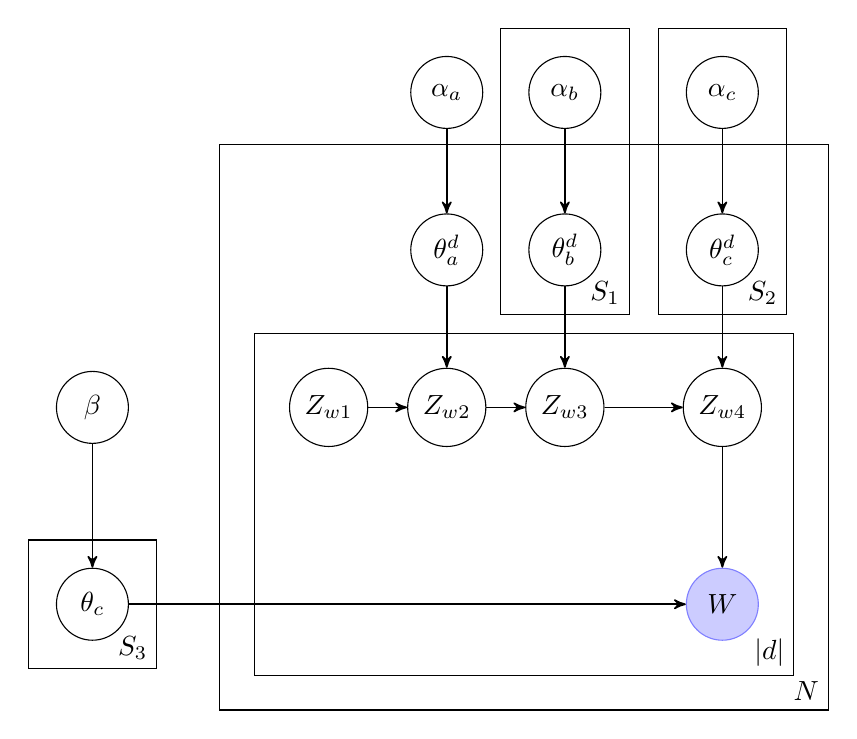
\begin{tikzpicture}
		[
		observed/.style={minimum size=26pt,circle,draw=blue!50,fill=blue!20},
		unobserved/.style={minimum size=26pt,circle,draw},
		post/.style={->,>=stealth',semithick},
		]
		
		\node (w-j) [observed] at (0,0) {$W$};
		\node (z-4) [unobserved, above of= w-j, node distance=2.5cm] {$Z_{w4}$};
		\node (z-3) [unobserved, left of= z-4, node distance=2cm] {$Z_{w3}$};
		\node (z-2) [unobserved, left of= z-3, node distance=1.5cm] {$Z_{w2}$};
		\node (z-1) [unobserved, left of= z-2, node distance=1.5cm] {$Z_{w1}$};
		
		\node (theta_a) [unobserved, above of= z-2, node distance=2cm] {$\theta_a^d$};
		\node (alpha_a) [unobserved, above of= theta_a , node distance=2cm] {$\alpha_a$};
		
		\node (theta_b) [unobserved, above of= z-3, node distance=2cm] {$\theta_b^d$};
		\node (alpha_b) [unobserved, above of= theta_b , node distance=2cm] {$\alpha_b$};
		
		\node (theta_c) [unobserved, above of= z-4, node distance=2cm] {$\theta_c^d$};
		\node (alpha_c) [unobserved, above of= theta_c , node distance=2cm] {$\alpha_c$};
		
		\node (theta_s2) [unobserved, left of=w-j , node distance=8cm] {$\theta_c$};
		\node (beta) [unobserved, above of=theta_s2 , node distance=2.5cm] {$\beta$};
		
		\path
		(z-4) edge [post] (w-j)
		(z-3) edge [post] (z-4)
		(z-2) edge [post] (z-3)
		(z-1) edge [post] (z-2)
		
		(theta_a) edge [post] (z-2)
		(alpha_a) edge [post] (theta_a)
		
		(theta_b) edge [post] (z-3)
		(alpha_b) edge [post] (theta_b)
		
		(theta_c) edge [post] (z-4)
		(alpha_c) edge [post] (theta_c)
		
		(theta_s2) edge [post] (w-j)
		(beta) edge [post] (theta_s2)
		;
		
		\node [draw,fit=(w-j) (theta_a) (z-1), inner sep=25pt] (plate-context) {};
		\node [above left] at (plate-context.south east) {$N$};
		
		\node [draw,fit=(w-j) (z-1), inner sep=12.5pt] (plate-token) {};
		\node [above left] at (plate-token.south east) {$|d|$};
		
		\node [draw,fit=(theta_s2), inner sep=10pt] (plate-token) {};
		\node [above left] at (plate-token.south east) {$S_3$};
		
		\node [draw,fit=(theta_c) (alpha_c), inner sep=10pt] (plate-token) {};
		\node [above left] at (plate-token.south east) {$S_2$};
		
		\node [draw,fit=(theta_b) (alpha_b), inner sep=10pt] (plate-token) {};
		\node [above left] at (plate-token.south east) {$S_1$};
		
	\end{tikzpicture}}
	\caption{Plate notation for the five-level \gls{pam}.}
	\label{fig:pachinko}
\end{figure}
\vejleder[inline]{a,b,c ~ $t_i$ in Figure 5}
				}
				\caption*{Five level Taxonomy-topic model}
			\end{figure}
		\end{column}
	\end{columns}
\end{frame}

\subsection{Results}

\begin{frame}{\insertsection}{Model Results}
	\begin{table}
		\centering
		\resizebox{.8\textwidth}{!}{
			\begin{tabular}{l|c|c}
				Topic Model & \makecell{Topic \\ Coherence} & \makecell{Topic \\ Difference} \\
				\midrule
				\Acrlong{lda} & 0.520 & 0.575 \\
				Author-topic model & 0.335 & 0.615 \\
				Category-topic model & 0.370 & 0.560 \\
				Taxonomy-topic model & \textbf{0.660} & \textbf{0.709} \\
			\end{tabular}
		}
	\end{table}
\end{frame}

\subsection{Other Notable Models}

\begin{frame}{\insertsubsection}{Quality comparison of \acrshort{pam} models}
	\centering
	\begin{tabular}{c|c|c|c|c|c|c}
		\makecell{Metadata \\ integration} & \multicolumn{5}{c}{\gls{dag} layer sizes} \vline & \makecell{Topic \\ Coherence} \\
		\hline
		$\checkmark$ & 1 & 4 & 32 & 90 & V & $0.66$\\
		- & & 1 & 100 & 90 & V & $0.67$ \\
	\end{tabular}
\end{frame}


\begin{frame}{\insertsubsection}{Time comparison of \acrshort{pam} models}
	\begin{tabular}{c|c|c|c|c|c|c}
		\makecell{Metadata \\ integration} & \multicolumn{5}{c}{\gls{dag} layer sizes} \vline & \makecell{Elapsed time \\ (hours)} \\
		\hline
		$\checkmark$ & 1 & 4 & 32 & 90 & V & 72 h\\
		$\crossmark$ & 1 & 4 & 32 & 90 & V & 83 h\\
		- & & 1 & 100 & 90 & V &  128 h\\
		- & 1 & 100 & 100 & 90 & V & $\sim 6300$ h\\
	\end{tabular}
\end{frame}

\begin{frame}{\insertsubsection}{Author-Category Model}
	\begin{figure}
		\centering
		\resizebox{0.3\columnwidth}{!}{%
			\begin{tikzpicture}
	[
	observed/.style={minimum size=26pt,circle,draw=blue!50,fill=blue!20},
	unobserved/.style={minimum size=26pt,circle,draw},
	post/.style={->,>=stealth',semithick},
	]
	
	\node (w-j) [observed] at (0,0) {$W_{d,n}$};
	\node (z-j) [unobserved, above of= w-j, node distance=2.5cm] {$Z_{d,n}$};
	\node (author_obs) [observed, above of= z-j, node distance=2.5cm] {${a_d, c_d}$};
	\node (author_dist) [unobserved, left of=z-j, node distance=2.5cm] {$\theta_a$};
	\node (category_dist) [unobserved, left of=author_obs, node distance=2.5cm] {$\theta_c$};
	\node (alpha-hyper) [unobserved, label=above:$\alpha$, above of=eta-hyper, node distance=3.75cm] {};
	\node (beta-hyper) [unobserved, left of = w-j, node distance=2.5cm] {$\beta_k$};
	\node (eta-hyper) [unobserved, label=above:$\eta$, left of=beta-hyper, node distance=2cm] {};
	
	\path
	(z-j) edge [post] (w-j)
	(alpha-hyper) edge [post] (author_dist)
	(alpha-hyper) edge [post] (category_dist)
	(category_dist) edge [post] (z-j)
	(author_obs) edge [post] (z-j)
	(author_dist) edge [post] (z-j)
	(beta-hyper) edge [post] (w-j)
	(eta-hyper) edge [post] (beta-hyper)
	;
	
	\node [draw,fit=(w-j) (author_obs), inner sep=14pt] (plate-context) {};
	\node [below right] at (plate-context.north west) {$D$};
	
	\node [draw,fit=(w-j) (z-j), inner sep=10pt] (plate-token) {};
	\node [below left] at (plate-token.north east) {$N$};
	
	\node [draw,fit=(beta-hyper) (beta-hyper), inner sep=17pt] (plate-context) {};
	\node [above right] at (plate-context.south west) {$K$};
	
	\node [draw,fit=(author_dist) (author_dist), inner sep=17pt] (plate-context) {};
	\node [above right] at (plate-context.south west) {$A$};
	
	\node [draw,fit=(category_dist) (category_dist), inner sep=17pt] (plate-context) {};
	\node [above right] at (plate-context.south west) {$C$};
	
\end{tikzpicture}
		}
	\end{figure}
	\begin{itemize}
		\item<1-> Topics are sampled from a combination of two topic proportions
		\item<2-> This setup makes it possible to view each of the metadata entry's topic distributions seperately
	\end{itemize}
\end{frame}

\begin{frame}{\insertsubsection}{Category-Doc Model}
	\begin{figure}
		\centering
		\resizebox{0.35\columnwidth}{!}{%
			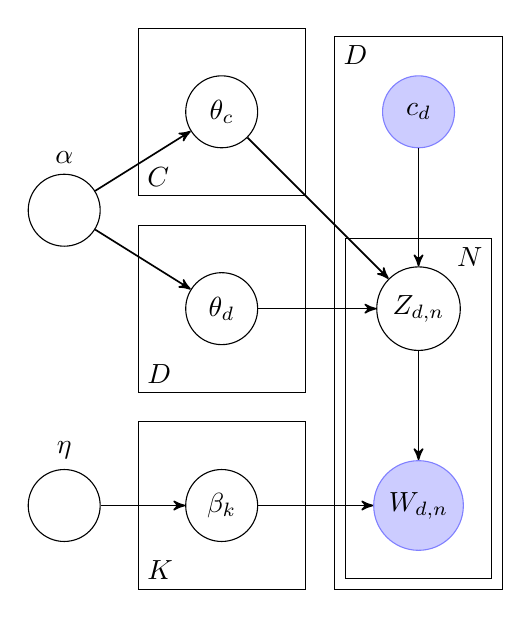
\begin{tikzpicture}
	[
	observed/.style={minimum size=26pt,circle,draw=blue!50,fill=blue!20},
	unobserved/.style={minimum size=26pt,circle,draw},
	post/.style={->,>=stealth',semithick},
	]
	
	\node (w-j) [observed] at (0,0) {$W_{d,n}$};
	\node (z-j) [unobserved, above of= w-j, node distance=2.5cm] {$Z_{d,n}$};
	\node (author_obs) [observed, above of= z-j, node distance=2.5cm] {${c_d}$};
	\node (author_dist) [unobserved, left of=z-j, node distance=2.5cm] {$\theta_d$};
	\node (category_dist) [unobserved, left of=author_obs, node distance=2.5cm] {$\theta_c$};
	\node (beta-hyper) [unobserved, left of = w-j, node distance=2.5cm] {$\beta_k$};
	\node (eta-hyper) [unobserved, label=above:$\eta$, left of=beta-hyper, node distance=2cm] {};
	\node (alpha-hyper) [unobserved, label=above:$\alpha$, above of=eta-hyper, node distance=3.75cm] {};
	
	\path
	(z-j) edge [post] (w-j)
	(alpha-hyper) edge [post] (author_dist)
	(alpha-hyper) edge [post] (category_dist)
	(category_dist) edge [post] (z-j)
	(author_obs) edge [post] (z-j)
	(author_dist) edge [post] (z-j)
	(beta-hyper) edge [post] (w-j)
	(eta-hyper) edge [post] (beta-hyper)
	;
	
	\node [draw,fit=(w-j) (author_obs), inner sep=14pt] (plate-context) {};
	\node [below right] at (plate-context.north west) {$D$};
	
	\node [draw,fit=(w-j) (z-j), inner sep=10pt] (plate-token) {};
	\node [below left] at (plate-token.north east) {$N$};
	
	\node [draw,fit=(beta-hyper) (beta-hyper), inner sep=17pt] (plate-context) {};
	\node [above right] at (plate-context.south west) {$K$};
	
	\node [draw,fit=(author_dist) (author_dist), inner sep=17pt] (plate-context) {};
	\node [above right] at (plate-context.south west) {$D$};
	
	\node [draw,fit=(category_dist) (category_dist), inner sep=17pt] (plate-context) {};
	\node [above right] at (plate-context.south west) {$C$};
	
\end{tikzpicture}
		}
	\end{figure}
	\begin{itemize}
		\item<1-> By having one topic-proportion for each document, one can combine the standard \gls{lda} with metadata models
	\end{itemize}
\end{frame}

\begin{frame}{\insertsubsection}{Combination model results}
	\begin{table}
		\centering
		\begin{tabular}{l|c|c}
			Topic Model & \makecell{Topic \\ Coherence} & \makecell{Topic \\ Difference} \\
			\midrule
			\Acrlong{lda} & 0.520 & 0.575 \\
			Author-topic model & 0.335 & 0.615 \\
			Category-topic model & 0.370 & 0.560 \\
			\textbf{Author-category model} & \textbf{0.390} & \textbf{0.537} \\
			\textbf{Author-doc model} & \textbf{0.543} & \textbf{0.574} \\
			\textbf{Category-doc model} &\textbf{ 0.530} & \textbf{0.575} \\
		\end{tabular}
	\end{table}
	\begin{itemize}
		\item<2-> Combining multiple topic-proportions can improve performance of topic models
		\item<3-> Having a topic proportion for each document, makes the performance similar to the standard \gls{lda}
	\end{itemize}
\end{frame}

%\begin{frame}{\insertsubsection}{Author-\acrshort{pam} \& Category-\acrshort{pam} Models}
%	Author-\gls{pam} and Category-\gls{pam} \gls{dag} structure:
%	\begin{itemize}
%		\item Single topic layer with locking mechanism
%		\item One topic for each author / category
%		\item Single topic layer with no locking mechanism
%	\end{itemize}
%	\only<2->{\begin{table}
%		\centering
%		\begin{tabular}{l|c}
%			Topic Model & \makecell{Topic \\ Coherence} \\
%			\midrule
%			\Acrlong{lda} & 0.520 \\
%			Author-topic model & 0.335 \\
%			Category-topic model & 0.370 \\
%			Taxonomy-topic model & 0.660 \\
%			\textbf{Author \gls{pam}} & \textbf{0.598} \\
%			\textbf{Category \gls{pam}} & \textbf{0.585} \\
%			\textbf{\Acrlong{pam}} & \textbf{0.670} \\
%		\end{tabular}
%	\end{table}}
%	\begin{itemize}
%		\item<3-> The \gls{pam} models achieve better performance than \gls{lda} models
%	\end{itemize}
%\end{frame}

%\section{Information Retrieval Methods}
%
%%part
%
%\begin{frame}{\insertsection}
%    \begin{itemize}
%        \item Latent Dirichlet Allocation (LDA)
%        \item PageRank (PR)
%        \item Language Model (LM)
%        \item Term Frequency - Inverse Document Frequency (TF-IDF)
%        \item Best Match 25 (BM25)
%    \end{itemize}
%\end{frame}
%
%\subsection{Latent Dirichlet Allocation}
%\begin{frame}{\insertsubsection}{Motivation}
%    %Produce a generative process with the best possible chance of reconstructing the existing documents, using topics.
%    \begin{itemize}
%        \item Create a generative process to produce documents, based on topics
%        \item Fine-tune to maximize probability of generating the original documents
%        \item Use generated topics for calculating similarity
%    \end{itemize}
%\end{frame}
%
%\begin{frame}{\insertsubsection}{Plate Notation}
%    \begin{figure}
%        \centering
%        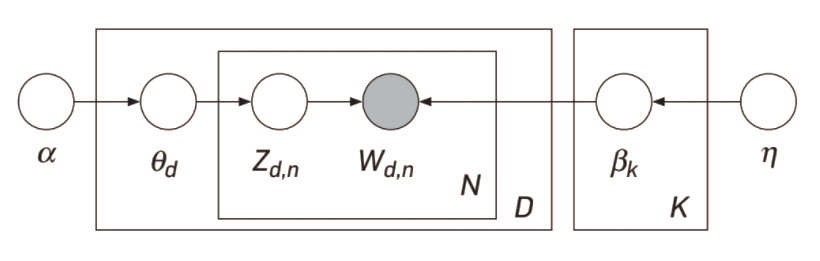
\includegraphics[width = 1 \textwidth]{figures/lda_model.jpg}
%    \end{figure}
%    \begin{itemize}
%        \item $\alpha, \eta$ dirichlet distributions
%        \item $\theta, \beta$ multinomial distributions
%        \item $Z, W$ sampled topics and words
%    \end{itemize}
%\end{frame}
%
%\begin{frame}{\insertsubsection}{Dirichlet Distributions}
%    \begin{figure}
%        \centering
%        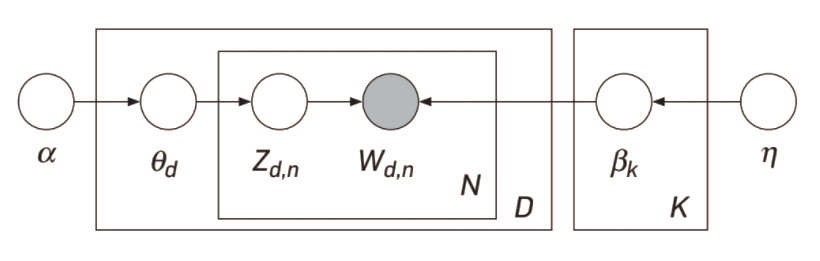
\includegraphics[width = 0.65 \textwidth]{figures/lda_model.jpg}
%    \end{figure}
%    \begin{figure}
%        \centering
%        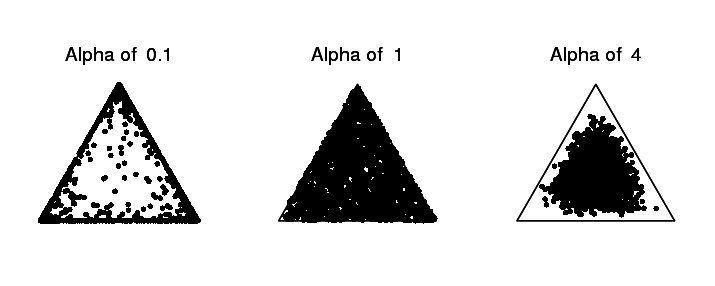
\includegraphics[width = 0.65 \textwidth]{figures/dirich.png}
%        \footnote{\url{https://mollermara.com/blog/lda/}}
%    \end{figure}
%    \begin{itemize}
%        \item<2> typical sample based on low alpha = $\{1,0,0\}$
%        \item<2> typical sample based on high alpha = $\{0.333, 0.333, 0.333\}$
%    \end{itemize}
%\end{frame}
%
%\begin{frame}{\insertsubsection}{Multinomial Distributions}
%    \begin{figure}
%        \centering
%        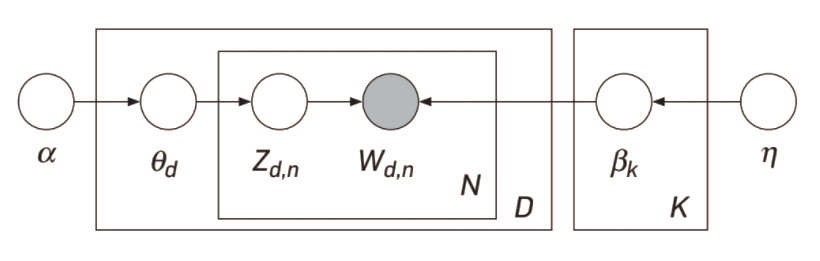
\includegraphics[width = 0.65 \textwidth]{figures/lda_model.jpg}
%    \end{figure}
%    \begin{itemize}
%        \item Sample $N$ topics ($Z$) based on $\theta$
%        \item Sample $N$ words ($W$) based on $Z$ and $\beta$
%    \end{itemize}
%\end{frame}
%
%\begin{frame}{\insertsubsection}{Generation Probability}
%    \begin{align*}
%        & P(W,Z,\theta,\beta;\alpha,\eta) = \\
%        & \prod_{d=1}^{D}P(\theta_d;\alpha)
%        \prod_{k=1}^{K}P(\beta_k;\eta)
%        \prod_{n=1}^{N}P(Z_{d,n}|\theta_d) P(W_{d,n}|\beta, Z_{d,n})
%    \end{align*}
%\end{frame}
%
%% full example?
%% training?
%
%\subsection{PageRank}
%\begin{frame}{\insertsubsection}{Overview}
%    \begin{itemize}
%        \item Used to rank nodes in a graph
%        \item Underlying assumption: important nodes have in-going connections from other important nodes
%        \item Based on the 'random surfer' model
%    \end{itemize}
%    \only<2>{\begin{figure}
%        \centering
%        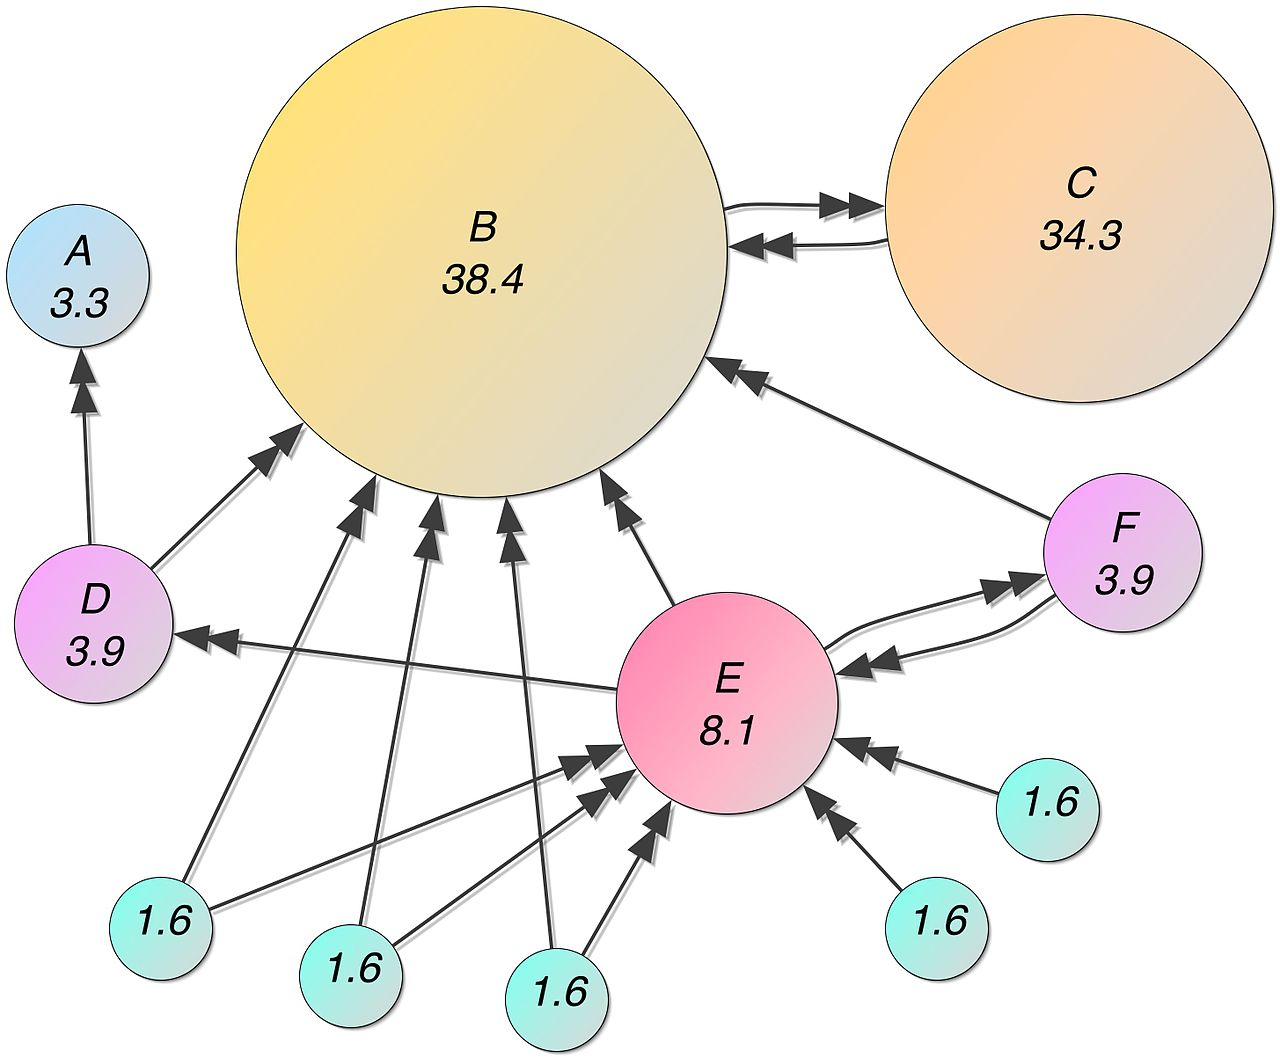
\includegraphics[width = 0.5 \textwidth]{figures/PageRank.jpg}
%        \footnote{\url{https://en.wikipedia.org/wiki/PageRank}}
%    \end{figure}}
%\end{frame}
%
%
%\begin{frame}{\insertsubsection}{Graph Construction}
%    \begin{itemize}
%        \item Used on adjacency matrix
%        \item Similarity between documents based on $\theta$
%        \begin{itemize}
%                    \item Calculated using Jensen-Shannon similarity
%        \end{itemize}
%        \item While fully connected each edge has a value which will influence the ranking
%    \end{itemize}
%\end{frame}

\section{Analysis}
\subsection{Author-topic \& category-topic models}
\begin{frame}{\insertsection}{\insertsubsection}
	\begin{block}{Category labels}
	    \begin{table}
	    	\centering
	    	\resizebox{.9\textwidth}{!}{
	    	\begin{tabular}{l|c|l|c|l|c}
	    		Category            & Number & Category        & Number & Category                       & Number  \\
	    		\midrule
	    		\cellcolor<2>{lightgray!75}Fælles              & 20204  &\cellcolor<2>{lightgray!75}Navne           &  3749  & \cellcolor<2>{lightgray!75}Kram                         &  244    \\
	    		\cellcolor<3>{lightgray!75}Thisted-avis        & 11473  & Kultur          &  3012  & misc                         &  229    \\
	    		Sport-avis          & 10941  & Morsø Sport     &  2350  & \cellcolor<1>{lightgray!75}53. Frederik                   &  203 \\
	    		Debat               & 10075  & \cellcolor<2>{lightgray!75}Friii           &  2333  & \cellcolor<2>{lightgray!75}Feature                        &  188 \\
	    		\cellcolor<3>{lightgray!75}Udland-avis         &  8855  & \cellcolor<2>{lightgray!75}Bagside         &  1933  &  &     \\
	    		Erhverv-avis        &  7356  & \cellcolor<2>{lightgray!75}MitLiv          &  1519  &  &     \\
	    		\cellcolor<3>{lightgray!75}Mariagerfjord-avis  &  7241  & \cellcolor<2>{lightgray!75}WEEKEND         &  1493  &  &     \\
	    		\cellcolor<3>{lightgray!75}Morsø-avis          &  5959  & Bo Godt         &  1447  &  &     \\
	    		\cellcolor<3>{lightgray!75}Aalborg-avis        &  5544  & Nordjyske Biler &  1400  &  &     \\
	    		\cellcolor<3>{lightgray!75}Vesthimmerland-avis &  5131  & Morsø Debat     &  1375  &  &     \\
	    		\cellcolor<3>{lightgray!75}Rebild-avis         &  4415  & \cellcolor<2>{lightgray!75}Frieord         &  1341  &  &     \\
	    		\cellcolor<3>{lightgray!75}Frederikshavn-avis  &  4325  & \cellcolor<2>{lightgray!75}Indsigt         &  984   &  &     \\
	    		\cellcolor<3>{lightgray!75}Hjørring-avis       &  4235  & Thisted sport   &  698   &  &     \\
	    		\cellcolor<3>{lightgray!75}Brønderslev-avis    &  3857  & \cellcolor<2>{lightgray!75}Perspektiv      &  613   &  &     \\
	    		\cellcolor<3>{lightgray!75}Jammerbugt-avis     &  3791  & \cellcolor<1>{lightgray!75}26. Frederik    &  484   &  &     \\
	    		\bottomrule
	    	\end{tabular}
    		}
	    \end{table}
	\end{block}
\end{frame}

\begin{frame}{\insertsection}{\insertsubsection}
	\begin{block}{Category similarity}
		\begin{table}
			\centering
			\resizebox{.7\textwidth}{!}{
			\begin{tabular}{r|c}
				Category pair & KL \\
				\midrule
				misc (292) \& Friii (2333) & 3.65 \\
				Friii (2333) \& Debat (10075) & 3.80 \\
				Feature (188) \& Hjørring-avis (4235) & 4.22 \\
				\rowcolor{lightgray!75} Sport-avis (10941) \& Morsø Sport (2350) & 5.04 \\
				Indsigt (984) \& Perspektiv (613) & 5.27 \\
				53. Frederik (203) \& Navne (3749) & 5.69 \\
				Rebild-avis (4415) \& Bo Godt (1447) & 5.78 \\
				Nordjyske Biler (1400) \& Thisted-avis (11473) & 5.91 \\
				misc (292) \& Debat (10075) & 6.67 \\
				Frederikshavn-avis (4325) \& Bo Godt (1447) & 6.81 \\
				\midrule
				Maximum KL divergence & 35.62 \\
				Median KL divergence & 27.09 \\
			\end{tabular}
			}
		\end{table}
	\end{block}
\end{frame}

\begin{frame}{\insertsection}{\insertsubsection}
	\begin{block}{Number of written articles}
		\begin{table}
			\centering
			\scriptsize
			\resizebox{.8\textwidth}{!}{
			\begin{tabular}{l|c|l|c}
				Author               & Number & Author                       & Number \\
				\midrule
				Ove Nørhave          &  9893  & AAArtikler parkeret          &   51   \\
				System Administrator &  9038  & Camilla Gammelgaard Johansen &   50   \\
				Ole Fink Mejlgaard   &  6518  & Klaus Færch Gjerulff         &   49   \\
				Peter Tordrup Larsen &  5002  & Ida Thorsen                  &   48   \\
				Kim Juhl Andersen    &  4506  & Mathias Overgaard            &   46   \\
				Jeppe Damsgaard      &  4057  & Kirsten Østergaard           &   45   \\
				Jørn Larsen          &  3863  & Gerda Buhl Andersen          &   44   \\
				Jørn Eriksen         &  3395  & Pia Christensen              &   44   \\
				Anders Kjærgaard     &  2960  & Dorte Rohde                  &   42   \\
				Søren Beukel Bak     &  2811  & Anna Grethe Jensen           &   41   \\
				Søren Olsson         &  2558  & Henrik Schulz                &   38   \\
				Jens Peter Svarrer   &  2480  & Lone Heilskov                &   37   \\
				Flemming Kristensen  &  2282  & Sarah Sandhøj                &   35   \\
				Thomas Jasper        &  2186  & Suzanne Tram                 &   34   \\
				Bente Lembo          &  2128  & Sebastian Engelberth Hansen  &   33   \\
				Helle Møller Larsen  &  1787  & Anna Østergaard Bjørn        &   29   \\
				Claus Jensen         &  1739  & Michael Sand Andersen        &   27   \\
				Esben Heine Pedersen &  1689  & HANNE Lindblad Jensen        &   27   \\
				Margit Sig           &  1632  & Mathilde Juul Back Jensen    &   25   \\
				Jens Fogh-Andersen   &  1614  & Allan Bauer                  &   19   \\
				Ole Jensen           &  1611  & Linse Daugaard               &   18   \\
				David Højmark        &  1549  & Morten Nis Klenø             &   17   \\
				Niels Hansen         &  1512  & OLE SANVIG KNUDSEN           &   16   \\
				Line Lykkegaard Skou &  1504  & Frederik Siiger              &   15   \\
				Lars Bang Bertelsen  &  1443  & Kim Lesanner                 &   15   \\
				\bottomrule
			\end{tabular}
			}
		\end{table}
	\end{block}
\end{frame}

\begin{frame}{\insertsection}{\insertsubsection}
	\begin{block}{Author similarity}
		\begin{table}
			\centering
			\resizebox{.8\textwidth}{!}{
			\begin{tabular}{r|c}
				Author pair & KL \\
				\midrule
				Lars Termansen (328) \& Mikkel Færgemann Viken (91) & 1.50 \\
				Morten Nis Klenø (17) \& Anne Helene Thomsen (606) & 1.72 \\
				Lars Termansen (328) \& Lars Christensen (1293) & 2.43 \\
				Esben Heine Pedersen (1689) \& Caspar Birk (71) & 2.47 \\
				Lars Christensen (1293) \& Poul Christoffersen (65) & 2.53 \\
				Lone Beck (92) \& Max Melgaard (587) & 2.74 \\
				HANNE Lindblad Jensen (27) \& Peter Tordrup Larsen (5002) & 2.94 \\
				Søren Kjær (95) \& Carl Chr. Madsen (785) & 2.98 \\
				Heidi Majgaard B. Pedersen (244) \& Lisbeth Helleskov (361) & 3.05 \\
				Lars Termansen (328) \& Morten Lind (413) & 3.16 \\
				\midrule
				Maximum & 34.51 \\
				Median & 24.20 \\
			\end{tabular}
			}
		\end{table}
	\end{block}
\end{frame}

\subsection{Taxonomy-topic model}
\begin{frame}{\insertsection}{\insertsubsection}
	\begin{block}{Similar topics in taxonomy-topic}
		\begin{table}
			\centering
			\resizebox{\textwidth}{!}{
			\begin{tabular}{c | c | c}
				Topic & Label & Top 10 words \\
				\midrule
				8 & politics & venstre, valg, valget, partiet, partier, parti, stemmer, mette, politik, regering \\
				9 & money & procent, viser, tal, antallet, milliarder, pct, seneste, penge, millioner, indland \\
				19 & filler & mig, maske, du, folk, synes, ting, faktisk, nogen, altid, tror \\
				\rowcolor{lightgray!75} 21 & university & unge, uddannelse, studerende, gymnasium, elever, uddannelser, universitet, procent, uddannelsen, nordjylland \\
				\rowcolor{lightgray!75} 41 & academic research & universitet, professor, forskere, forskning, forskerne, viser, verden, institut, procent, aarhus \\
				42 & filler & mig, min, mit, ham, aldrig, gik, lille, maske, mine, altid \\
				45 & wildlife & dyr, naturen, natur, ulve, fugle, ulven, arter, dyrene, vilde, ulv \\
				47 & church & kirke, kirken, sognepræst, præst, søndag, koret, gudstjeneste, aften, kor, organist \\
				59 & music concerts & musik, koncert, sange, spiller, koncerter, band, koncerten, festival, musikken, publikum \\
				60 & buisness & virksomheden, millioner, a, direktør, procent, medarbejdere, selskabet, overskud, ansatte, virksomhed \\
				\rowcolor{lightgray!75} 69 & primary school & elever, unge, skole, eleverne, skolen, skoler, klasse, børn, folkeskolen, lærere \\
				74 & elder care & ældre, borgere, kommunen, millioner, penge, nordjylland, plejehjem, borgerne, kommunens, budget \\
				75 & filler & du, din, dig, dit, altsa, dine, maske, nemlig, bruge, hvordan \\
				79 & filler & mig, min, hendes, hende, rigtig, arige, altid, arbejde, mor, mine \\
				86 & sports & handbold, mors, thy, hold, kamp, sæson, kampe, kampen, point, holdet \\
			\end{tabular}
			}
		\end{table}
	\end{block}
\end{frame}

\begin{frame}{\insertsection}{\insertsubsection}
	\begin{block}{Filler topics in taxonomy-topic}
		\begin{table}
			\centering
			\resizebox{\textwidth}{!}{
				\begin{tabular}{c | c | c}
					Topic & Label & Top 10 words \\
					\midrule
					8 & politics & venstre, valg, valget, partiet, partier, parti, stemmer, mette, politik, regering \\
					9 & money & procent, viser, tal, antallet, milliarder, pct, seneste, penge, millioner, indland \\
					\rowcolor{lightgray!75} 19 & filler & mig, maske, du, folk, synes, ting, faktisk, nogen, altid, tror \\
					21 & university & unge, uddannelse, studerende, gymnasium, elever, uddannelser, universitet, procent, uddannelsen, nordjylland \\
					41 & academic research & universitet, professor, forskere, forskning, forskerne, viser, verden, institut, procent, aarhus \\
					\rowcolor{lightgray!75} 42 & filler & mig, min, mit, ham, aldrig, gik, lille, maske, mine, altid \\
					45 & wildlife & dyr, naturen, natur, ulve, fugle, ulven, arter, dyrene, vilde, ulv \\
					47 & church & kirke, kirken, sognepræst, præst, søndag, koret, gudstjeneste, aften, kor, organist \\
					59 & music concerts & musik, koncert, sange, spiller, koncerter, band, koncerten, festival, musikken, publikum \\
					60 & buisness & virksomheden, millioner, a, direktør, procent, medarbejdere, selskabet, overskud, ansatte, virksomhed \\
					69 & primary school & elever, unge, skole, eleverne, skolen, skoler, klasse, børn, folkeskolen, lærere \\
					74 & elder care & ældre, borgere, kommunen, millioner, penge, nordjylland, plejehjem, borgerne, kommunens, budget \\
					\rowcolor{lightgray!75} 75 & filler & du, din, dig, dit, altsa, dine, maske, nemlig, bruge, hvordan \\
					\rowcolor{lightgray!75} 79 & filler & mig, min, hendes, hende, rigtig, arige, altid, arbejde, mor, mine \\
					86 & sports & handbold, mors, thy, hold, kamp, sæson, kampe, kampen, point, holdet \\
				\end{tabular}
			}
		\end{table}
	\end{block}
\end{frame}

\section{Conclusion}
\begin{frame}{\insertsection}{}
	\begin{itemize}
		\item \textit{How can we establish models that incorporate metadata from the Nordjyske dataset?}
		\begin{itemize}
			\item<2-> Adapting \gls{lda} and the \gls{pam}
			\item<2-> Usable for multiple metadata types
		\end{itemize}
	\vspace{.2cm}
		\item \textit{How does including metadata within such models impact the resulting topics?}
		\begin{itemize}
			\item<3-> Depends on the model and dataset
			\item<3-> New model distributions give new possibilities
		\end{itemize}
	\end{itemize}
\end{frame}
%%%%%%%%%%%%%%%%

{\aauwavesbg
\begin{frame}[plain,noframenumbering]
  \finalpage{Thank you}
\end{frame}}
%%%%%%%%%%%%%%%%


\end{document}